\chapter{Inertia and Cascading Failures}

\label{ch:contribution}


Hopefully after reading Chapter \ref{ch:cf}, it is clear that numerous models exist to quantify a power system's risk to cascading failure, but very little research has been done to understand the role of a power system's inertia during cascading failures.  Cascading failures and power system inertia have largely been treated as separate issues in the literature, but it is intuitive to believe that decreasing the system's ability to respond to instabilities will change its security from larger cascades.  A thorough understanding of the interplay between the transient dynamics and cascade response is specifically lacking from the literature.  For the proposed work, I will address what I believe to be two separate issues in regards to inertia: the first is how \textit{total} system inertia affects cascade dynamics, the second is how the \textit{distribution} of inertia affects cascades.


First, we need to understand how total system inertia impacts stability and risk of failure.  As a reminder, total system inertia is a weighted average of every generator's inertia constant and its rated apparent power output $$ H_{tot} = \frac{\sum_{i=1}^{n_g} H_i S_{B_i}}{\sum_{i=1}^{n_g} S_{B_i}} $$ and is independent of the system's topology.  This parameter is related to a power system's total kinetic energy, and decreasing inertia lowers a system's ability to respond quickly to failures, and maintain a balance between power generation and consumption.  The motivation for studying how total system inertia influences stability comes from recent regulations on a maximum amount of inertia-less generation at any given time, for example in Ireland [CITE].  It is unclear what value of total system inertia is necessary to maintain stability, thus we will explore the effect of decreasing total system inertia on the system's risk to cascading failure.  This will be investigated by incrementally reducing total system inertia and running cascading failure simulations ($n-1$ and $n-2$ contingencies to start) and observing how the distribution of failures changes as total system inertia changes.  While this is not how a power system's total inertia will actually change, it separates out the effect of decreasing inertia from where inertia is actually located on the grid.

Second, we would like to understand how the distribution of inertia changes power system stability.  Consider two scenarios shown in Figure \ref{fig:inertia_dist}.  The first illustrates a network with evenly distributed inertia, while the second illustrates a case where all inertia generators are in one area of the system, while all inertia-less generators are in another area of the power system.  We wish to explore the difference in stability between these two cases.  where all generators with inertia are at one end of a system, and all generators without inertia are at another end of a system.  This allows us to specifically address the interplay between topology and dynamics.  In particular, is there a relation between the severity of a cascade and the distribution of inertia on the system?  To address this question we will need to first quantify what the distribution of inertia is on a power system.  Let $D_P$ be the diameter of the power system in question, and $\sigma(i,g)$ be the shortest path between a bus $i$ and a generator $g$, then we define the total kinetic energy absorbed at bus $i$ as


\begin{equation}
KE_i = \frac{1}{\sum_{\forall g \in G}KE_g}\sum_{\forall g \in G}KE_g\frac{\sigma (i,g)}{D_P}
\label{eqtn:ke_bus}
\end{equation}

We can quantify the severity of a cascade in a multitude of ways, the more prominent choices in the literature are cascade size (in terms of number of failed lines, or amount of load shed).  We will use the number of failed lines in this work, but we also choose to explore a few other measures which include the amount 

\section{Model for Cascading Failure}

To study the effect of inertia on power system stability during cascading failures, it is important to use a model that not only accurately reflects the cascading failure dynamics, but also the transient dynamics of the generators.  For this reason, we choose to run the cascading failure simulations using the continuous phase-space (CPS) model developed in \cite{Yang2017} and [Cite DEMARCO].  It is important to note that this model assumes constant voltage magnitudes at every bus, and does not solve for reactive power.  We previously discussed that voltage stability is very important for maintaining reliability, and thus this is a limitation of the CPS model.  For this reason, we will compare results obtained with the continuous model to the results from PSLF, a commercial software created by General Electric, which is an industry standard for testing power system stability.  We expect that the results of some cascades will be different between the two models, but we hypothesize that the continuous model should never be worse than the PSLF model, as the PSLF model accounts for more potential instabilities than the continuous model.  The purpose of using the continuous model is to understand the usefulness of the lyapunov energy function to the understanding of cascade severity and outcome.  However, should the results differ significantly (i.e. in terms of the number of outages, or size of frequency deviations), then we will use the final results from PSLF, because it is the industry standard. Additionally, the comparison of these two models will serve as an exploration into the accuracy of the DC power flow approximation compared to the AC power flow equations.  

\section{Power Networks to Use}

This section is going to explain which power system test cases I am going to use and why.

In order to study inertial impacts, I will use two specific test cases.  The first is a model of the Central Illinois power system, and the second is a model of the ERCOT test case.  Both of these models were created using population information of specific zip codes for creating load data, and statistical information about generators from the Energy Information Administration \cite{Birchfield2017}.  The generator dynamic data, such as damping and inertial constants, are drawn from a distribution of known inertia constants for generators of different types, such as coal or nuclear \cite{Xu2017}. 




%To explain why this is important, consider the IEEE Iceland test case system, which consists of 189 buses, 203 power lines, and 35 generators.  A plot of $n-k$ failures, up to $k=3$ is shown in Figure \ref{fig:n_k_iceland}.  Unsurprisingly, larger failures become more likely as the number of simultaneous outages increases, but a more interesting feature is the slight bi-modality shown for all $n-k$ test runs.  This is most likely due to the fact that a power system is a finite network, and thus estimating cascade size based on infinite size networks, or probabilistic cascade models does not accurately reflect the risk of failure \cite{Burkholz2018}\cite{Schafer2018}.  The bi-modality could also be a result of adding generator dynamics to the cascade model, which is a strong hypothesis when we observe a similar trend using the IEEE New-England transmission system with the COSMIC model \cite{cosmic}.
%This justifies a study of a finite set of possible outages for a particular network under specific load and generation scenarios for a deeper understanding of how generator dynamics affect cascade outcomes.

%As we discussed in Chapters \ref{ch:intro} and \ref{ch:background}, power systems are growing in complexity with the addition of renewable generation.  A large area of focus is the effect of lower inertia in the system, and how this effects the transient dynamics after a perturbation.  Based on Figure [INSERT FIGURE COMPARING n-k outages for different inertia values], we can see (hopefully that probability distribution is not all that different.)  Additionally, the energy distribution values are also not that different.  This is consistent with the conclusion reached in \cite{Manik2014}, that the inertia constant $M$, does not influence \textit{where} stable operating points are, but it does change which outages can reach those operating points.  Part of this work will try to understand how the addition of renewable resources influences specific cascades, and why some events are more unstable, while some are less unstable.  We will do this by exploring the inertia parameters of the Iceland network using the continuous phase-space cascade model, and using the Western Wind and Solar Integration Study (WWSIS) Phase III WECC model created by NREL using the commercial software PSLF \cite{Miller2014}. 
%
%The WWSIS model was developed by NREL in collaboration with numerous industry partners to understand if the Western Interconnection could handle larger penetrations of solar and wind generation, and how it would perform under various scenarios.  It is the largest renewable integration study to date, and includes details of the network topology, generator dynamics, and renewable resource availability. [Add some other stuff about what it entails].
%
%As we noted in Chapter \ref{ch:cf}, an under explored model of cascading failure associates a Lyapunov energy function with the cascading failure process.  Figure \ref{fig:energy_iceland} shows the energy levels of the Iceland network using the model described in \cite{Yang2017}.  Very strong clustering around a few energy values is observed, but this is not correlated with the number of outages that occurred during the cascade.  Therefore, we hypothesize that this clustering could be the result of a few scenarios. (I) The network dynamics cause certain transmission lines to fail together, which creates a discretization in the energy levels.  (II) Particular network configurations are more stable than others, and each energy level is a manifestation of a stable network configuration.  (III) A combination of (I) and (II).
%
%
%
%\begin{figure}
%\centering
%\label{fig:n_k_iceland}
%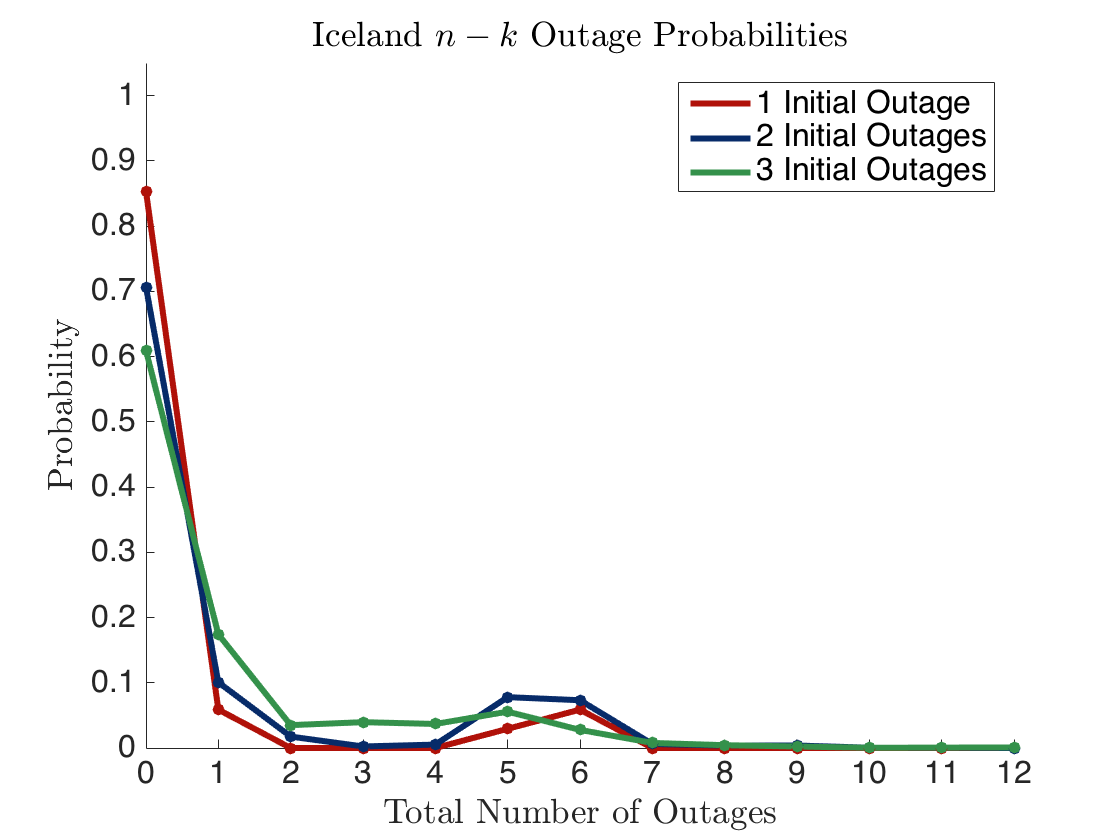
\includegraphics[width=0.8\textwidth]{figures/iceland_probs}
%\caption{Distribution of outages for the Icelandic test network using the continuous phase-space model.  Total number of outages does not include the initial $k$ outages.}
%\end{figure}
%
%
%\begin{figure}
%\centering
%\label{fig:energy_iceland}
%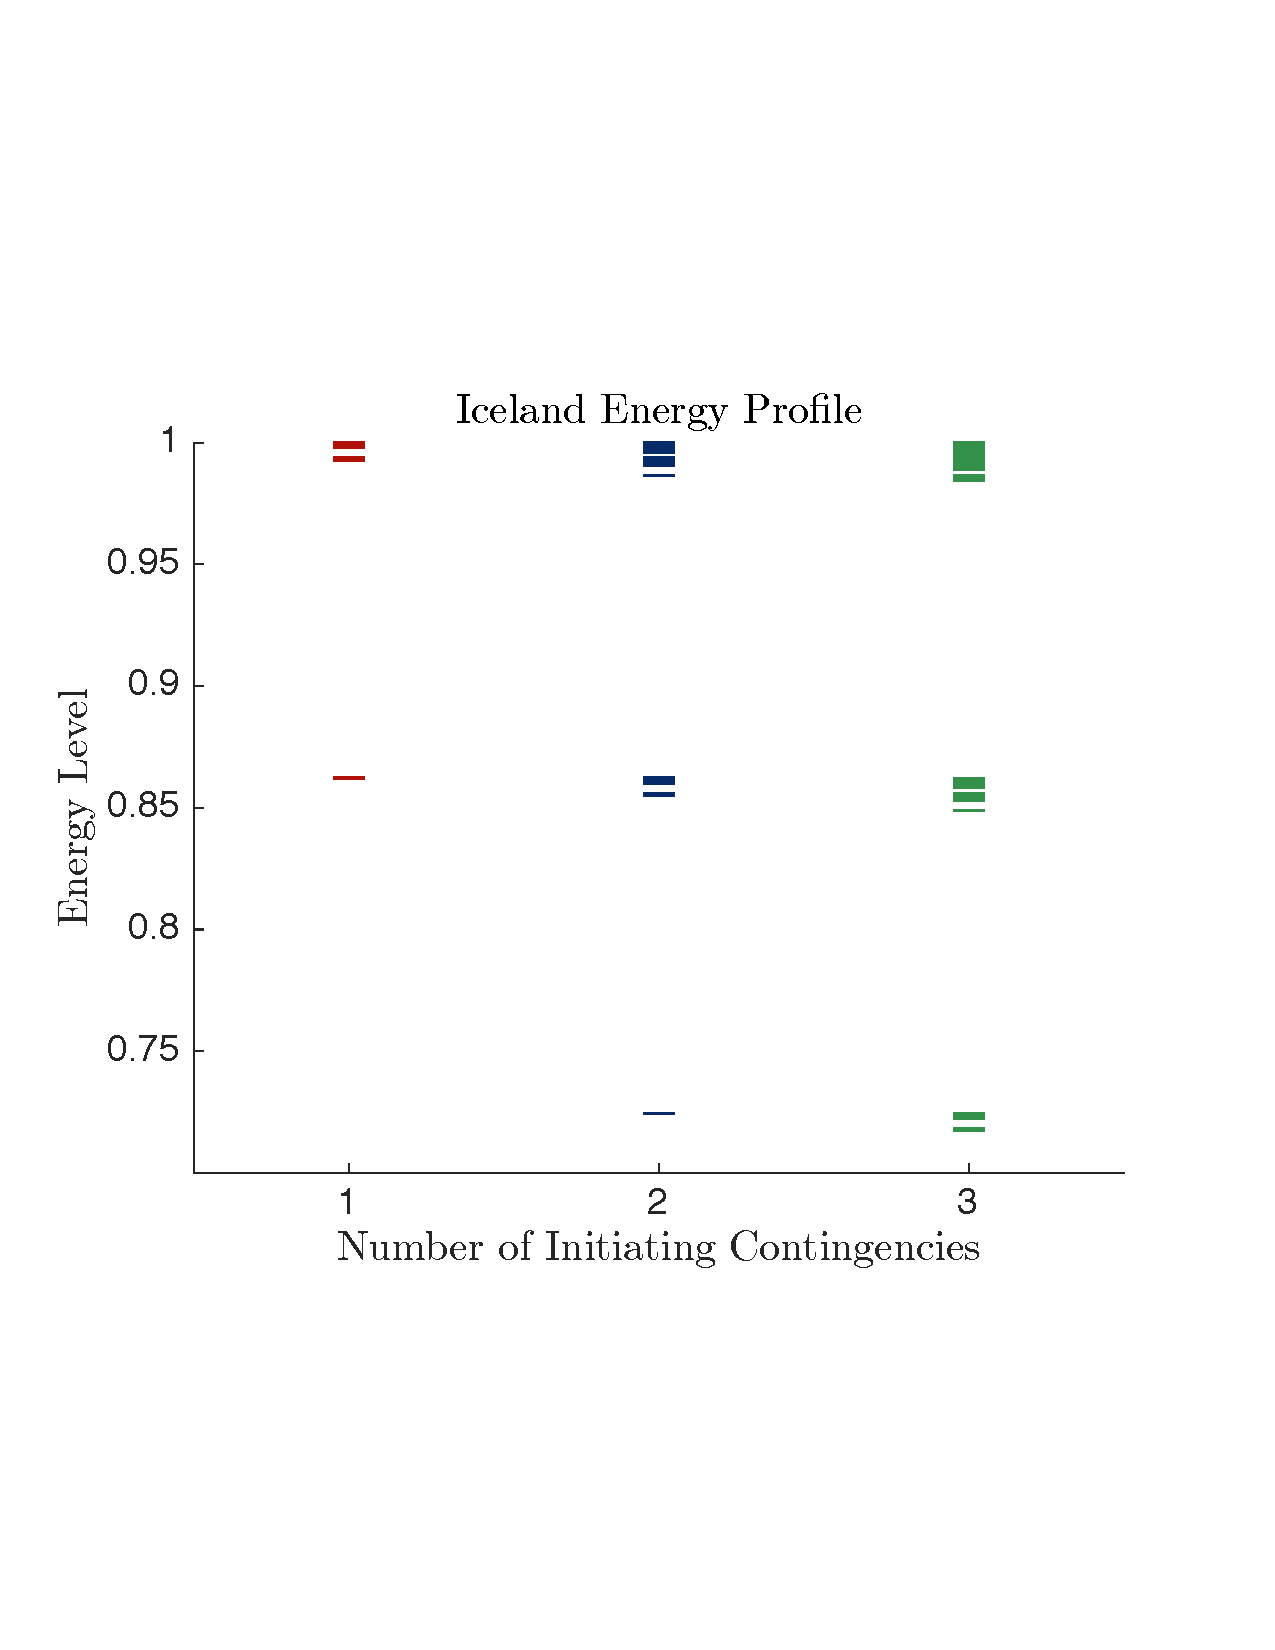
\includegraphics[width=0.7\textwidth]{figures/iceland_energy.pdf}
%\caption{Distribution of energy levels for the Icelandic test network using the continuous phase-space model.  Energy level is a fraction of the energy level of the stable network.}
%\end{figure}
%
%
%The goal of this thesis is to understand which explanation (I)-(III), best explains this clustering phenomenon.  First, it will be important to determine if the clustering continues for larger values of $k$, at least up to $k=4$, but ideally up to $k=5$.  If the clustering trend does in fact continue, then this provides strong evidence that (I)-(III) could be valid reasons for the phenomenon.  To determine which of (I)-(III) applies, we will analyze the cascade results in the following way.  First, we will determine the conditional probabilities of line $j$ failing, given that line $i$ failed, in a similar manner presented in \cite{hines_ig} and \cite{YangCoSep}.  This will give us a sense of the dependency of line failures.  To test (II), we will perform motif analysis, which counts the occurrence of small substructures of a larger network [CITATION].  This has mostly been applied to gene regulatory networks, but cascading failure analysis has been moving towards this direction of research for a while, with the use of $k$-core analysis and   the study of the effects of dead-ends on grid stability \cite{kurths2014}\cite{YangMotterSVS}.
%
%



















